\chapter{\texorpdfstring{$\mr{P}_2$}{$\mr{P}_2$}上的函数的Lions导数}
本章内容主要参考引用自\citep{MFG}的5.2节.\par
记$\mr{P}$表示$\mb{R}^d$上全体概率测度,$\mr{P}_p$表示全体$p$阶矩有限概率测度,即
$$
\mr{P}_p=\{\mu\in\mr{P}:\int_{\mb{R}^d}\abs{x}^p\mu(\mathrm{d}x)<\infty\}.
$$
$\mr{P}_p$在$p-$Wasserstein距离$W_p(\cdot,\cdot)$下是一个完备度量空间,$W_p(\cdot,\cdot)$定义为
$$
W_p(\mu,\nu)\coloneq \inf_{\pi\in\Pi(\mu,\nu)}(\int_{\mb{R}^d\times\mb{R}^d} \abs{x-y}^p\pi(\mathrm{d}x,\mathrm{d}y))^{\frac{1}{p}},
$$
其中$\Pi(\mu,\nu)$表示所有边缘分布为$\mu,\nu$的联合分布.本章中如无特别说明,总默认$\mathscr{P}_2$配备$W_2(\cdot,\cdot)$距离及其诱导的度量拓扑.
称$\mathscr{P}_2$的子集$K$是有界的,是指:存在$R>0$,使得$\forall \mu\in K,\int_{\mathbb{R}^d}\abs{x}^2 \mathrm{d}\mu(x)\leq R$.
\par
对一个函数$f:\mr{P}_2\to\mb{R}$,我们希望考察$\mu\in\mr{P}_2$处的局部性态,但由于$\mr{P}_2$不是Banach空间,
甚至不是向量空间,所以不能直接使用第一章中的Frechet导数和Gateaux导数.Lions导数的想法是不直接考察概率测度$\mu$附近函数的性态,
而是考虑将$f$先"提升"为定义在$L^2(\Omega,\mr{F},\mb{P};\mb{R}^d)$上的函数$\tilde{f}$,考察分布为$\mu$的随机变量
$X\in L^2(\Omega,\mr{F},\mb{P};\mb{R}^d)$附近$\tilde{f}$的性态,而$L^2(\Omega,\mr{F},\mb{P};\mb{R}^d)$不仅是Banach空间,
也是Hilbert空间,所以可以应用Frechet可微性的概念.一个自然的提升是令$\tilde{f}=f\circ\mr{L}$,其中$\mr{L}(X)$
表示$\mb{R}^d$上由随机变量$X$诱导的概率分布,也即$\mr{L}(X)(A)=\mb{P}(X^{-1}(A)),\forall A\in\mr{B}(\mb{R}^d)$.

\[
    \begin{tikzcd}
X \arrow[rrrr, maps to]                                                &  &  &                     & \mu=\mr{L}(X) \arrow[dddd, maps to] \\
L^2(\Omega,\mr{F},\mb{P};\mb{R}^d) \arrow[rrr, "\mr{L}" description] \arrow[rrrddd, "\tilde{f}=f\circ\mr{L}" description, dashed] &  &  & B \arrow[ddd, "f"description] &                         \\
                                                                       &  &  &                     &                         \\
                                                                       &  &  &                     &                         \\
                                                                       &  &  & \mb{R}                   & f(\mu)                      
\end{tikzcd}
\]\par
由\citep{Boga}的命题9.1.11,对于任意的无原子的概率空间,任意分布$\mu\in\mr{P}$,总存在一个随机变量$X$使得$\mr{L}(X)=\mu$,这一事实
保证了提升的合理性.本章讨论提升时,无原子的概率空间$(\Omega,\mr{F},\mb{P})$总是固定的,简记$L^2(\Omega;\mb{R}^d)=L^2(\Omega,\mr{F},\mb{P};\mb{R}^d)$.
对任意$A\in \mr{F}$,记$\mr{F}|_A\coloneq \{E\cap A:E\in \mr{F}\}$.
另外,在本章中,对于一个Banach空间$B$上的函数$F$,不加区分的使用$F'(a)$和$DF(a)$表示$F$在$a\in B$
处的Frechet导数,同样地,若有定义,不加区分地使用$F'$和$DF$表示$F$的导数映射.
\section{L-可微性}
\subsection{定义}
\begin{definition}
    给定一个函数$f:\mr{P}_2\to \mb{R}$,称$f$在$\mu_0\in\mr{P}_2$是L-可微的,是指:存在一个分布为$\mu_0$的随机变量$X_0$,
    使得$f$的提升$\tilde{f}=f\circ\mr{L}:L^2(\Omega;\mb{R}^d)\to\mb{R}$在$X_0$处是Frechet可微的.
\end{definition}\par
这个定义的表述是自然的,但良定性并不显然,具体地说,对于同一个概率测度,可能有多个随机变量以其为分布,那么
就需要说明这些随机变量和其Frechet导数有某种不变量或者在某种等价关系下属于同一等价类,使得定义在一定的标准下具有唯一性.为此,我们先陈述以下引理.\par
\begin{lemma}\label{lm3.1}
    设$X,Y\in L^2(\Omega;\mb{R}^d)$分布相同.则对任意$\epsilon>0$,存在保测映射\footnote{设$(X_1,\mr{F}_1,\mu_1),(X_2,\mr{F}_2,\mu_2)$是两个测度空间
    ,称$M:(X_1,\mr{F}_1,\mu_1)\to(X_2,\mr{F}_2,\mu_2)$是一个保测映射,是指:$M$可测且任意$A\in\mr{F}_2,\mu_2(A)=\mu_1(M^{-1}(A))$.}$S,T:\Omega\to\Omega$使得
    $$
    \mb{P}(\{\omega\in\Omega:(S\circ T)(\omega)=(T\circ S)(\omega)=\omega\})=1
    $$且
    $$
    \mb{P}(\abs{Y-X\circ T}\leq \epsilon)=1.
    $$
\end{lemma}
\begin{proof}[证明梗概] 
    记$\mr{F}^*,\mb{P}^*$分别为$\mr{F},\mb{P}$的完备化扩张.\par
    对给定的$\epsilon$,设$\{A_n\}_{n=1}^\infty\subset\mr{B}(\mb{R}^d)$是$\mb{R}^d$的一个剖分,且任意$A_n$直径不超过$\epsilon$(例如边长为$\frac{\epsilon}{\sqrt{d}}$的半开半闭的方体).
    令$B_n=X^{-1}(A_n),C_n=Y^{-1}(A_n)$,由于$X,Y$同分布,所以$\mb{P}(B_n)=\mb{P}(C_n)$.不妨设$\mb{P}(B_n)>0$.
    由于$(\Omega,\mr{F},\mb{P})$无原子,所以存在$M_n\subset\tilde{M}_n\subset B_n,N_n\subset\tilde{N}_n\subset C_n$,$\mb{P}(\tilde{M_n})=\mb{P}(\tilde{N_n})=0$.\par
    记$\Omega_n^X=B_n-M_n,\mr{F}_n^X=\{A\cap\Omega_n^X:A\in\mr{F}^*\},\mb{P}_n^X(E)=\frac{\mb{P}^*(E)}{\mb{P}(B_n)},E\in\mr{F}_n^X$以及$\Omega_n^Y=C_n-N_n,\mr{F}_n^Y=\{A\cap\Omega_n^Y:A\in\mr{F}^*\},\mb{P}_n^Y(E)=\frac{\mb{P}^*(F)}{\mb{P}(C_n)},F\in\mr{F}_n^Y$.\par
    由\citep{Boga}的推论6.6.7和定理9.2.2可知,存在保测的双射
    $$
    \tilde{S}_n:(\Omega_n^X,\mr{F}^X_n,\mb{P}^X_n)\to (\Omega_n^Y,\mr{F}^Y_n,\mb{P}^Y_n).
    $$和
    $$
    \tilde{T}_n:(\Omega_n^Y,\mr{F}^Y_n,\mb{P}^Y_n)\to (\Omega_n^X,\mr{F}^X_n,\mb{P}^X_n)
    $$且$\tilde{S}_n\circ \tilde{T}_n=\mathrm{id}_{\Omega_n^X},\tilde{T}_n\circ \tilde{S}_n=\mathrm{id}_{\Omega_n^Y}$.



\tikzset{every picture/.style={line width=0.75pt}} 

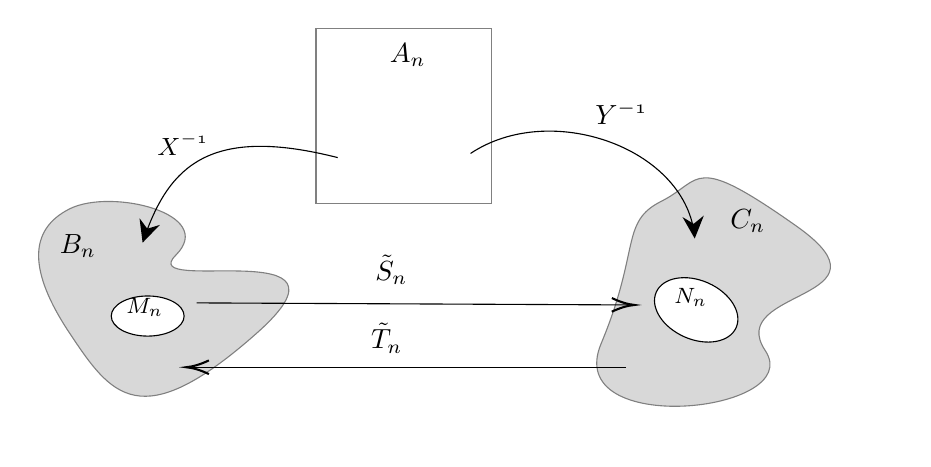
\begin{tikzpicture}[x=0.75pt,y=0.75pt,yscale=-1,xscale=1]
%uncomment if require: \path (0,300); %set diagram left start at 0, and has height of 300

%Shape: Square [id:dp04833006195011558] 
\draw  [color={rgb, 255:red, 128; green, 128; blue, 128 }  ,draw opacity=1 ] (187.67,52) -- (272,52) -- (272,136.33) -- (187.67,136.33) -- cycle ;
%Shape: Polygon Curved [id:ds1886656269714927] 
\draw  [color={rgb, 255:red, 128; green, 128; blue, 128 }  ,draw opacity=1 ][fill={rgb, 255:red, 155; green, 155; blue, 155 }  ,fill opacity=0.39 ] (354.11,135.33) .. controls (374.11,125.33) and (368.11,111.33) .. (419.11,147.33) .. controls (470.11,183.33) and (384.11,177.33) .. (404.11,207.33) .. controls (424.11,237.33) and (305.89,249.67) .. (325,204) .. controls (344.11,158.33) and (334.11,145.33) .. (354.11,135.33) -- cycle ;
%Shape: Polygon Curved [id:ds9357130005520881] 
\draw  [color={rgb, 255:red, 128; green, 128; blue, 128 }  ,draw opacity=1 ][fill={rgb, 255:red, 155; green, 155; blue, 155 }  ,fill opacity=0.39 ] (69,139) .. controls (89,129) and (140.11,141.33) .. (120.11,161.33) .. controls (100.11,181.33) and (215.11,149.33) .. (159,199) .. controls (102.89,248.67) and (89,229) .. (69,199) .. controls (49,169) and (49,149) .. (69,139) -- cycle ;
%Curve Lines [id:da5137408307588414] 
\draw    (262.11,112.33) .. controls (300.33,86.85) and (364.48,109.39) .. (369.86,150.78) ;
\draw [shift={(370.11,153.33)}, rotate = 266.01] [fill={rgb, 255:red, 0; green, 0; blue, 0 }  ][line width=0.08]  [draw opacity=0] (10.72,-5.15) -- (0,0) -- (10.72,5.15) -- (7.12,0) -- cycle    ;
%Curve Lines [id:da15386414272233362] 
\draw    (198.11,114.33) .. controls (136.69,98.73) and (117.09,118.31) .. (105.02,152.66) ;
\draw [shift={(104.11,155.33)}, rotate = 288.43] [fill={rgb, 255:red, 0; green, 0; blue, 0 }  ][line width=0.08]  [draw opacity=0] (10.72,-5.15) -- (0,0) -- (10.72,5.15) -- (7.12,0) -- cycle    ;
%Shape: Ellipse [id:dp9061451224593543] 
\draw  [fill={rgb, 255:red, 255; green, 255; blue, 255 }  ,fill opacity=1 ] (89,190.67) .. controls (89,185.33) and (96.86,181) .. (106.56,181) .. controls (116.25,181) and (124.11,185.33) .. (124.11,190.67) .. controls (124.11,196.01) and (116.25,200.33) .. (106.56,200.33) .. controls (96.86,200.33) and (89,196.01) .. (89,190.67) -- cycle ;
%Shape: Ellipse [id:dp31508727833906336] 
\draw  [fill={rgb, 255:red, 255; green, 255; blue, 255 }  ,fill opacity=1 ] (351.58,179.16) .. controls (354.75,172) and (365.94,170.03) .. (376.57,174.74) .. controls (387.2,179.46) and (393.24,189.08) .. (390.07,196.24) .. controls (386.89,203.39) and (375.7,205.37) .. (365.08,200.65) .. controls (354.45,195.93) and (348.4,186.31) .. (351.58,179.16) -- cycle ;
%Straight Lines [id:da9603829886778048] 
\draw    (130.11,184.33) -- (339.11,185.32) ;
\draw [shift={(341.11,185.33)}, rotate = 180.27] [color={rgb, 255:red, 0; green, 0; blue, 0 }  ][line width=0.75]    (10.93,-3.29) .. controls (6.95,-1.4) and (3.31,-0.3) .. (0,0) .. controls (3.31,0.3) and (6.95,1.4) .. (10.93,3.29)   ;
%Straight Lines [id:da7009166377859317] 
\draw    (337.11,215.33) -- (127.11,215.33) ;
\draw [shift={(125.11,215.33)}, rotate = 360] [color={rgb, 255:red, 0; green, 0; blue, 0 }  ][line width=0.75]    (10.93,-3.29) .. controls (6.95,-1.4) and (3.31,-0.3) .. (0,0) .. controls (3.31,0.3) and (6.95,1.4) .. (10.93,3.29)   ;
% Plotting does not support converting to Tikz

% Text Node
\draw (222,58) node [anchor=north west][inner sep=0.75pt]   [align=left] {$\displaystyle A_{n}$};
% Text Node
\draw (63,150) node [anchor=north west][inner sep=0.75pt]   [align=left] {$\displaystyle B_{n}$};
% Text Node
\draw (386,138) node [anchor=north west][inner sep=0.75pt]   [align=left] {$\displaystyle C_{n}$};
% Text Node
\draw (95,181) node [anchor=north west][inner sep=0.75pt]  [font=\footnotesize] [align=left] {$\displaystyle M_{n}$};
% Text Node
\draw (359,176) node [anchor=north west][inner sep=0.75pt]  [font=\footnotesize] [align=left] {$\displaystyle N_{n}$};
% Text Node
\draw (215,160) node [anchor=north west][inner sep=0.75pt]   [align=left] {$\displaystyle \tilde{S}_{n}$};
% Text Node
\draw (213,193) node [anchor=north west][inner sep=0.75pt]   [align=left] {$\displaystyle \tilde{T}_n$};
% Text Node
\draw (110,101) node [anchor=north west][inner sep=0.75pt]  [font=\small] [align=left] {$\displaystyle \mathnormal{X^{-1}}$};
% Text Node
\draw (321,86) node [anchor=north west][inner sep=0.75pt]   [align=left] {$\displaystyle \mathnormal{Y^{-1}}$};


\end{tikzpicture}\par
下面把$\tilde{S}_n,\tilde{T}_n$从$B_n-\tilde{M}_n,C_n-\tilde{N}_n$延拓到$B_n,C_n$上,记为$S_n,T_n$.只需补充在$\tilde{M}_n,\tilde{N}_n$上的定义,具体地说,任取$x_n\in M_n,y_n\in N_n$,
令$\forall x\in \tilde{M}_n,S_n(x)=y_n,\forall y\in \tilde{N}_n,T_n(y)=x_n$即可.容易验证,延拓后的映射$S_n$是$(B_n,\mr{F}|_{B_n})$
到$(C_n,\mr{F}|_{C_n})$的保测映射.$T_n$类似.\par
当$\mb{P}(B_n)=0$时,取$M_n=B_n,N_n=C_n$.\par
令$S=\sum_{n\geq 1} S_n I_{B_n},T=\sum_{n\geq 1} T_n I_{C_n}$,则$S,T$是
$(\Omega,\mr{F},\mb{P})$到自身的保测映射.且以概率1互为逆.\par
最后,对几乎处处$\omega$,存在$n$,使得$\omega\in C_n$,则$T(\omega)\in B_n$,所以$X(T(\omega)),Y(\omega)\in A_n$.
\end{proof}

因为$L^2(\Omega;\mb{R}^d)$是一个Hilbert空间,所以对函数$F:L^2(\Omega;\mb{R}^d)\to \mb{R}$在一点
$X$处的Frechet导数$DF(X)$作为一个Hilbert空间的对偶空间的元素,总可以视为$L^2(\Omega;\mb{R}^d)$中的某个随机变量,对任意$Y\in L^2(\Omega;\mb{R}^d)$
的作用以$DF(X)(Y)=\langle DF(X),Y\rangle=\mb{E}[DF(X)\cdot Y]$的形式表现.

\begin{theorem}
    设函数$f:\mr{P}_2\to \mb{R}$在$\mu_0\in\mr{P}_2$处L-可微.则对于任意分布为$\mu_0$的随机变量
    $X\in L^2(\Omega;\mb{R}^d)$,$f$的提升$\tilde{f}$在$X$处是Frechet可微的,且$(X,D\tilde{f}(X))$的联合分布
    不依赖于$X$的选取.
\end{theorem}
\begin{proof}
    由定义,存在分布为$\mu$的随机变量$X_0\in L^2(\Omega;\mb{R}^d)$,$\tilde{f}$在$X_0$处是Frechet可微的.
    对任意分布为$\mu$的随机变量$X\in L^2(\Omega;\mb{R}^d)$,任意$\epsilon>0$,存在$\Omega$到自身的保测映射$S_\epsilon$和$T_\epsilon$
    满足
    $$
    \mb{P}(\{\omega\in\Omega:S(T(\omega))=T(S(\omega))=\omega\})=1
    $$和
    $$
    \mb{P}(\abs{X_0-X\circ S}\leq \epsilon)=1.
    $$
    注意到$\tilde{f}$作为$f$的提升,其函数值只依赖于随机变量的分布,所以对任意$Y\in L^2(\Omega;\mb{R}^d)$,
    \begin{align}
        \tilde{f}(X+Y)&=\tilde{f}((X+Y)\circ S_\epsilon)\notag\\
        &=\tilde{f}(X_0+(X\circ S_\epsilon-X_0)+Y\circ S_\epsilon)\notag\\
        &=\tilde{f}(X_0)+(\tilde{f})'(X_0)((X\circ S_\epsilon-X_0)+Y\circ S_\epsilon)\notag\\
        &\quad+\nm[L^2]{(X\circ S_\epsilon-X_0)+Y\circ S_\epsilon}\delta((X\circ S_\epsilon-X_0)+Y\circ S_\epsilon)\notag\\
        &=\tilde{f}(X_0)+\mb{E}[D\tilde{f}(X_0)\cdot ((X\circ S_\epsilon-X_0)+Y\circ S_\epsilon)]\notag\\
        &\quad+\nm[L^2]{(X\circ S_\epsilon-X_0)+Y\circ S_\epsilon}\delta((X\circ S_\epsilon-X_0)+Y\circ S_\epsilon)\notag\\
        &=\tilde{f}(X)+\mb{E}[(D\tilde{f}(X_0)\circ T_\epsilon)\cdot Y]+\mb{E}[D\td{f}(X_0)\cdot (X\circ S_\epsilon-X_0)]\notag\\
        &\quad+\nm[L^2]{(X\circ S_\epsilon-X_0)+Y\circ S_\epsilon}\delta((X\circ S_\epsilon-X_0)+Y\circ S_\epsilon).
    \end{align}
    其中$\delta(\cdot)$与$\epsilon$无关且$\lim_{\nm[L^2]{Y}\to 0} \delta(Y)=0$,第1个等号和第5个等号
    分别使用了$S_\epsilon,T_\epsilon$的保测性.\par
    取$\epsilon=\frac{1}{n},n\in \mb{N}$,记$Z_n=D\td{f}(X_0)\circ T_{\frac{1}{n}}$.由式(3.1)可得
    $$
    \mb{E}[(Z_n-Z-m)\cdot Y]\leq C(\abs{\frac{1}{n}-\frac{1}{m}}+o(\nm[L^2]{Y})),
    $$
    所以$\{Z_n\}$会在$L^2(\Omega;\mb{R}^d))$中收敛到某个随机变量,最后在式(3.1)中令$\epsilon\to 0$即可.
\end{proof}
L-可微性的定义是将定义域从一个概率测度组成的空间转换到一个随机变量空间上讨论的,但应该注意到$f:\mr{P}_2\to \mb{R}$
在一点处的局部性态应该只和该点和其周围的概率测度决定,下面的定理将说明L-可微性确实是函数的内蕴性质,并对Lions导数给出
一个稍微独立于随机变量的表示.在此之前,首先引入连续L-可微的概念,这是连续Frechet可微的自然延伸,称$f:\mr{P}_2\to \mb{R}$
是连续L-可微的,是指:$f$在任意$\mu\in\mr{P}_2$处是L-可微的,且$D\td{f}(X)$是以$X$为自变量的从$L^2(\Omega;\mb{R}_d)$到自身的连续映射.

\begin{theorem}\label{3.3}
    设$f:\mr{P}_2\to \mb{R}$是连续L-可微的.则对任意$\mu\in\mr{P}_2$,存在可测函数$\xi:\mb{R}_d\to \mb{R}_d$,使得任意以
    $\mu$为分布的随机变量$X$,都有$D\td{f}(X)=\xi(X)$.
\end{theorem}
\begin{proof}
    对给定的$X$,首先证明$D\td{f}(X)$关于$X$生成的$\sigma$代数$\sigma(X)$可测.不妨设$f$有界.证明分为以下几步.\par
    (1)\ 先考虑$\mu$关于Lebsgue测度绝对连续,且对$\forall q>4$,$\mu(\abs{\cdot}^q)<\infty$.对$\epsilon>0$,
    定义
    $$
    \Psi(Y)=\td{f}(Y)+\frac{1}{2\epsilon}\mathbb{E}[\abs{X-Y}^2]+\mathbb{E}[\abs{Y}^4],\quad Y\in L^4(\Omega;\mathbb{R}^d),
    $$
    则$\Psi$在$L^4(\Omega;\mathbb{R}^d)$是Frechet可微的,且任意$Y\in L^4(\Omega;\mathbb{R}^d)$,
    $$
    \Psi'(Y)=D\td(f)(Y)+\frac{1}{\epsilon}(Y-X)+4 \mathbb{E}[\abs{Y}^2]Y.
    $$
    由于$\Psi$有下界,从而一定有下确界,取$\{Z_n\}\subset L^4(\Omega;\mathbb{R}^d)$为$\Psi$的极小化序列,即$\lim_{n\to \infty}\Psi(Z_n)=\inf_{Z\in L^4(\Omega;\mathbb{R}^d)}\Psi(Z)$以及
    $\nu_n=\mathscr{L}(\nu_n)$.由Brenier定理(陈述及证明可见\citep{figot}的定理2.5.10),存在一列$\mathbb{R}^d$上的凸函数$\{\psi_n\}$满足
    $\mathscr{L}(\nabla\psi(X_n))=\nu_n$且是$\mu-$a.e.可微的,此外还有$W_2(\mu,\nu_n)=\mathbb{E}[\abs{X-\nabla\psi(X_n)}^2]$.记$Y_n=\nabla\psi(X_n)$,
    则
    \begin{align}
        \Psi(Y_n)&=\td{f}(Y_n)+\frac{1}{2\epsilon}W_2(\mu,\nu_n)^2+\mathbb{E}[\abs{Y}^4]\leq \Psi(Z_n),
    \end{align}
    从而$\{Y_n\}$也是$\Psi$的一个极小化序列.\par
    而$
    \sup_{n\geq 1} \nu_n(\abs{\cdot}^4)\infty$,结合Chebyshev不等式
    可得$\{\nu_n\}$是胎紧的.不妨设$\nu_n$在$W_2$距离和弱收敛意义下收敛到$\nu$,所以
    \begin{align}
        &f(\nu)=\lim_{n\to\infty} f(\nu),\notag\\
        &W_2(\mu,\nu)=\lim_{n\to\infty} W_2(\mu,\nu_n).\notag\\
    \end{align}\par
    由Fatou引理的测度收敛版本(见\citep{bogawc}的推论2.2.6)可得
    $$
    \int_{\mathbb{R}^d} \abs{x}^4\nu(\mathrm{d}x)\leq \liminf_{n\to\infty}\mathbb{E}[\abs{Y}^4]<\infty.
    $$
    再次利用Brenier定理可得,存在凸函数$\psi:\mathbb{R}^d\to \mathbb{R}$使得$Y\coloneq \nabla\psi(X)$分布为$\nu$且
    $W_2(\mu,\nu)=\mathbb{E}[\abs{X-Y}^2]$.因为$\Psi$在$Y$处取得极小值,由\citep{FA2}的定理7.1-5知$D\Psi(Y)=0$.
    即
    $$
    D\td{f}(Y)=-\frac{1}{\epsilon}(Y-X)-4\abs{Y}^2Y,
    $$
    这说明$D\td{f}(Y)\in\sigma(X)$.\par
    注意到这里的$Y$是依赖于$\epsilon$的,不妨记为$Y_\epsilon$,由于$Y_\epsilon$极小化$\Psi_\epsilon$,
    所以对任意$\epsilon$,
    $$\mathbb{E}[\abs{X-Y_\epsilon}^2]\leq 2(\td{f}(X)+\mathbb{E}[\abs{X}^4]-(\td{f}(Y_\epsilon)+\mathbb{E}[\abs{Y_\epsilon}^4])),
    $$
    所以令$\epsilon\to 0$,$Y_\epsilon\to X$.这就证得了$D\td{f}(X)\in\sigma(X)$.\par
    (2)\ 假设$\mu\in \mathscr{P}_2$关于Lebsgue测度绝对连续但不一定有(1)中的矩条件,取分布为$\mu$的随机变量$X\in L^2(\Omega;\mathbb{R}^d)$,
    令$X_n=\frac{nX}{\sqrt{n^2+X^2}}$,再令$n\to\infty$即可.\par
    (3)\ 若$\mu\in \mathscr{P}_2$不是关于Lebsgue测度绝对连续的,取分布为$\mu$的随机变量$X\in L^2(\Omega;\mathbb{R}^d)$和$\Omega$上两个独立的标准正态分布的
    随机变量$N_1,N_2$,且$X$独立于$N_1,N_2$.令$X_{n,i}=X+\frac{1}{n}N_i,n\in \mathbb{N},i=1,2$,则$X_{n,i}$的分布总是关于Lebsgue测度绝对连续的,从而可得
    $D\td{f}(X)\in \sigma(X,N_i)$,而由$N_1,N_2$的独立性,可得$D\td{f}(X)\in\sigma(X)$.\par
    最后我们说明$\xi$不依赖于$X$的选取.假设对两个分布为$\mu$的二阶矩有限随机变量$X_1,X_2$分别有对应的
    $\xi_1,\xi_2$,任取$A\in\mathscr{B}(\mathbb{R}^d)$,易见$\mu(\xi_1 I_A)=\mu(\xi_2 I_A)$,所以$\xi_1=\xi_2,\mu-$a.e..
\end{proof}
有了以上定理,我们可以借助概率空间和随机变量给出L-可微函数$f:\mathscr{P}_2\to \mathbb{R}$在$\mu_0$处的局部性态:
$$
f(\mu)=f(\mu_0)+\mathbb{E}[D\td{f}(X_0)\cdot (X-X_0)]+o(\nm[L^2]{X-X_0}),
$$
其中$\mathscr{L}(X)=\mu,\mathscr{L}(X_0)=\mu_0$.\par
另一方面,为了突出L-可微的内蕴性,我们将定理\ref{3.3}中的$\xi$记为$\partial_\mu f(\mu_0)$,称为$f$在
$\mu_0$处的Lions导数或L-导数.此时有
\begin{equation}\label{diffor}
    f(\mu)=f(\mu_0)+\mathbb{E}[\partial_\mu f(\mu_0)(X_0)\cdot (X-X_0)]+o(\nm[L^2]{X-X_0}),
\end{equation}

其中$\mathscr{L}(X)=\mu,\mathscr{L}(X_0)=\mu_0$.

作为以上微分公式的一个应用,给出如下命题,这是\citep{brw}的定理2.1的特殊情形.
\begin{corollary}\label{cr1}
    设函数$f:\mathscr{P}_2\to \mathbb{R}$连续,在一个无原子的概率测度$\mu_0$处L-可微,存在常数$C$使得
    \[
        \abs{\partial_{\mu}f(\mu_0)(x)}\leq C(1+\abs{x}).
    \]
    $(X_s)_{s\in[0,1]}\subset L^2(\Omega;\mathbb{R}^d)$是一族随机变量,$\mathscr{L}(X_0)=\mu_0$,$X_s$关于$s$连续,且
    $\dot{X}_0\coloneq \lim_{s\downarrow} \frac{X_s-X_0}{s}$在$L^2(\Omega;\mathbb{R}^d)$中存在.则
    \[
        \lim_{s\downarrow 0}\frac{f(\mathscr{L}(X_s))-f(\mu_0)}{s}=\mathbb{E}[\ipr{\partial_{\mu}f(\mu_0)(X_0) }{\dot{X}_0}].
    \]
\end{corollary}
\subsection{若干例子}
\begin{example}[线性函数]\label{eg3.1}
    我们首先计算积分形式给出的线性函数.给定光滑函数$h:\mathbb{R}^d\to \mathbb{R}$,且$\abs{\nabla h(x)}\leq C(1+\abs{x})$.
    令$f(\mu)=\int_{\mathbb{R}^d} h(x)\mu(\mathrm{d}x)$,$f$的提升为$\td{f}(X)=\mathbb{E}[h(X)]$,其中$\mathscr{L}(X)=\mu$.
    计算$\td{f}$的Frechet导数,首先由中值定理,
    \begin{equation}
        h(x+y)=h(x)+\int_0^1 (\nabla h(x+ty)\cdot y) \mathrm{d}t,
    \end{equation}
    \begin{equation}
        \begin{aligned}
            \mathbb{E}[h(X+Y)]&=\mathbb{E}[h(X)+\int_0^1 (\nabla h(X+tY)\cdot Y) \mathrm{d}t]\\
            &=\mathbb{E}[h(X)]+\mathbb{E}[\nabla h(X)\cdot Y]+\mathbb{E}[\int_0^1 (\nabla h(X+tY)\cdot Y-\nabla h(X)\cdot Y) \mathrm{d}t],
        \end{aligned}
    \end{equation}
    其中,
    \begin{equation}
        \begin{aligned}
            &\abs{\mathbb{E}[\int_0^1 \bra{(\nabla h(X+tY)-\nabla h(X))\cdot Y}\mathrm{d}t]}\\
            \leq&\int_0^1 \mathbb{E}[\bra{((\nabla h(X+tY)-\nabla h(X))\cdot Y)} I_{\{\abs{Y}\leq \nm[L^2]{Y}^{1/2}\}}]\mathrm{d}t\\
            &\quad +\int_0^1 \mathbb{E}[\bra{((\nabla h(X+tY)-\nabla h(X))\cdot Y)} I_{\{\abs{Y}> \nm[L^2]{Y}^{1/2}\}}]\mathrm{d}t\\
            \leq&\mathbb{E}[\sup_{y\leq \nm[L^2]{Y}^{1/2}} \bra{\nabla h(X+y)-\nabla h(X)}]\nm[L^2]{Y}\\
            &\quad +C'\mathbb{E}[(1+\abs{X}+\abs{Y})\abs{Y}]\\
            \leq&\mathbb{E}[\sup_{y\leq \nm[L^2]{Y}^{1/2}} \bra{\nabla h(X+y)-\nabla h(X)}]\nm[L^2]{Y}\\
            &\quad +C'\nm[L^2]{Y}(\nm[L^2]{Y}+\nm[L^2]{Y}^{1/2}+\sup_{\mathbb{P}(A)\leq \nm[L^2]]{Y}} \mathbb{E}[\abs{X}^2 I_A]^{1/2})
        \end{aligned}
    \end{equation}
    所以$\partial_\mu f(\mu)=\nabla h,\forall \mu\in \mathscr{P}_2$.\par
    这个例子虽然简单,但也说明了Lions导数和古典导数以及Frechet导数的一些区别:尽管对线性函数,其L-导数仍然是
    固定的,但并非$h$,而是其梯度.
\end{example}
\begin{example}[续例\ref{eg3.1},卷积函数]
    接下来考虑一个稍微复杂的函数,令$h*\mu (x)=\int_{\mathbb{R}^d} h(x-y)\mu(\mathrm{d}y)$,$g(\mu)=f(h*\mu)$.易见
    $\td{g}(X)=\int_{\mathbb{R}^d} \mathbb{E}[h(x-X)]\mathrm{d}\mathscr{L}(X)(x)$,由第一章相关讨论可知,当$\td{g}$在一点Frechet
    可微时,为了确定该点处的Frechet导数,只需计算所有的Gateaux导数,所以先计算$X$处沿$Y$方向的Gateaux导数,

    \begin{equation}
        \begin{aligned}
            &\td{g}(X+\epsilon Y)-\td{g}(X)\\
            =&\int_{\mathbb{R}^d} \mathbb{E}[h(x-(X+\epsilon Y))]\mathrm{d}\mathscr{L}(X+\epsilon Y)(x)-\int_{\mathbb{R}^d} \mathbb{E}[h(x-X)]\mathrm{d}\mathscr{L}(X)(x)\\
            =&\bra{\int_{\mathbb{R}^d} \mathbb{E}[h(x-X-\epsilon Y)]\mathrm{d}\mathscr{L}(X+\epsilon Y)(x)-\int_{\mathbb{R}^d} \mathbb{E}[h(x-X)]\mathrm{d}\mathscr{L}(X+\epsilon Y)(x)}\\
            &\quad +\bra{\int_{\mathbb{R}^d} \mathbb{E}[h(x-X)]\mathrm{d}\mathscr{L}(X+\epsilon Y)(x)-\int_{\mathbb{R}^d} \mathbb{E}[h(x-X)]\mathrm{d}\mathscr{L}(X)(x)}\\
            \overset{\triangle}{=}& I_1+I_2,
        \end{aligned}
    \end{equation}
    对于第二项,结合Fubini定理交换积分次序可得
    $$
    \lim_{\epsilon\to 0}\frac{I_2}{\epsilon} =\int_{\mathbb{R}^d}\mathbb{E}[\nabla h(x-X)\cdot Y]\mathrm{d}\mathscr{L}(X)(x),
    $$
    而对于第一项,取$(X,Y)$的一个独立复制$(\hat{X},\hat{Y})$,
    则\begin{equation}
        \begin{aligned}
            I_1&=\mathbb{E}[h((\hat{X}+\epsilon \hat{Y})-(X+\epsilon Y))]-\mathbb{E}[h(\hat{X}+\epsilon \hat{Y}-X)]\\
            &=\mathbb{E}[h((\hat{X}+\epsilon \hat{Y})-(X+\epsilon Y))]-\mathbb{E}[h(\hat{X}-X)]\\
            &\quad +\mathbb{E}[h(\hat{X}-X)]-\mathbb{E}[h(\hat{X}+\epsilon \hat{Y}-X)],
        \end{aligned}
    \end{equation}
    所以
    $$
    \lim_{\epsilon\to 0}\frac{I_2}{\epsilon}=\mathbb{E}[\nabla h(\hat{X}-X)\cdot(\hat{Y}-Y)]-\mathbb{E}[\nabla h(\hat{X}-X)\cdot(\hat{Y})]=-\mathbb{E}[\nabla h(\hat{X}-X)\cdot Y].
    $$\par
    综上可得,$\partial_\mu g(\mu)=(\nabla(h+\bar{h}))*\mu$,其中$\bar{h}(x)\coloneq h(-x)$.

\end{example}

\begin{example}\label{eg3.3}
    考虑连续函数$v:\mathbb{R}^d\times \to \mathscr{P}_2$满足:\par
(1)\ $\forall \mu\in \mathscr{P}_2$,$v(x,\mu)$关于$x$可微,记$\nabla v(x,\mu)$表示$v$在$(x,\mu)$
处关于$x$的梯度.任意有界集$K\subset \mathscr{P}_2$,存在常数$C_1$,使得任意$\mu\in K,\abs{\nabla v(x,\mu)}\leq C_1(1+\abs{x})$.\par
(2)\ 任意$\mu\in \mathscr{P}_2,x\in \mathbb{R}^d$,使得$(x,y)\mapsto $可测,且$\partial_\mu v(x,\mu)(y)$关于$y$连续,并且对任意
有界集$K\subset \mathscr{P}_2$,存在常数$C_2$,使得任意$\mu\in K$,$\partial_\mu v(x,\mu)(y)\leq C_2(1+\abs{y})$.\par
令$u(\mu)=\int_{\mathbb{R}^d} v(x,\mu)\mathrm{d}\mu(x)$,计算$u$的Lions导数,计算中由于涉及到多个随机变量,因此在合适的时候应该回到函数的定义
以免造成混淆.首先注意到$u$的提升$\td{u}(X)=\mathbb{E}[v(X,\mathscr{L}(X))]$,
\begin{equation}
    \begin{aligned}
        &\td{u}(X+Y)-\td{u}(X)\\
        =&\mathbb{E}[v(X+Y,\mathscr{L}(X+Y))]-\mathbb{E}[v(X,\mathscr{L}(X))]\\
        =&\mathbb{E}[v(X+Y,\mathscr{L}(X+Y))]-\mathbb{E}[v(X,\mathscr{L}(X+Y))]\\
        &\quad+\mathbb{E}[v(X,\mathscr{L}(X+Y))]-\mathbb{E}[v(X,\mathscr{L}(X))]\\
        \overset{\triangle}{=}&I_1+I_2,
    \end{aligned}
\end{equation}
由中值定理可得,
$$
I_1=\mathbb{E}[\int_0^1 \nabla v(X+tY,\mathscr{L}(X+Y))\cdot Y \mathrm{d}t)],
$$
而
\begin{equation}
    \begin{aligned}
        I_2&=\int_{\mathbb{R}^d} (v(x,\mathscr{L}(X+Y))-v(x,\mathscr{L}(X)))\mathrm{d}\mathscr{L}(X)(x)\\
        &=\int_{\mathbb{R}^d} \int_0^1 \mathbb{E}[\partial_\mu v(x,\mathscr{L}(X+tY))(X+tY)\cdot Y]\mathrm{d}t \mathrm{d}\mathscr{L}(X)(x),
    \end{aligned}
    \notag
\end{equation}
所以可以合理推测$\partial_\mu f(\mu)(\cdot)=\nabla v(\cdot,\mu)+\int_{\mathbb{R}^d} \partial_\mu f(y,\mu)(\cdot)\mathrm{d}\mu(y)$,事实上根据对
$v$的假设,采用和例\ref{eg3.1}中类似的讨论方法可知,$f$在$\mu$处的L-导数确实为上式.
\end{example}

\begin{example}[续\ref{eg3.3}]
    设$K:\mathbb{R}^d\times \mathbb{R}^d\to \mathbb{R}^d$为一可测映射,$\nabla_1 K,\nabla_2 K$分别表示对第1个和第2个自变量的梯度,且都是至多线性增长的,
    令$v(x,\mu)=\int_{\mathbb{R}^d} K(x,y)\mathrm{d}\mu(y)$,则由上例结果可得
    $$
    \partial_\mu f(\mu)(x)=\int_{\mathbb{R}^d}(\nabla_1 K(x,y)+\nabla_1 K(y,x))\mathrm{d}\mu(y).
    $$
    
\end{example}

\section{链式法则和It\^{o}公式}
给定一个完备的带流概率空间$(\Omega,(\mathscr{F}_t)_{t\geq 0},\mathbb{P})$和其上的一个$m$维的$\mathscr{F}_t-$布朗运动$(B_s)_{s\geq 0}$,设$\mathscr{F}_t$是右连续的,即
$\mathscr{F}_{t+}\coloneq \cap_{s>t} \mathscr{F}_s =\mathscr{F}_t$,$(b_t)_{t\geq 0},(\sigma_t)_{t\geq 0}$分别为$\Omega$上
$\mathbb{R}^d$和$\mathbb{R}^{d\times m}$值的循序可测过程,$X_0\in L^2(\Omega,\mathscr{F}_0,\mathbb{P};\mathbb{R}^d)$,且对任意$T>0$都有
$$
\mathbb{E}[\int_0^T (\abs{b_t}^2+\nm[HS]{\sigma_t}^4) \mathrm{d}t]<\infty,
$$其中$\nm[HS]{\sigma_s}\coloneq \sqrt{\tr(a_s)}\coloneq \sqrt{\tr (\sigma_s \sigma_s^*)}$.令
\begin{align}\label{itopro}
    X_t=X_0+\int_0^t b_s \mathrm{d}s+\int_0^t \sigma_s \mathrm{d}B_s,\quad t\geq 0.
\end{align}
对于式(3.10)给出的Ito过程和任一$\mathbb{R}^d$上的二次连续可微函数$f$,都有Ito公式
\begin{equation}\label{itofor}
f(X_t)=f(X_0)+\int_0^t \nabla f(X_s)\cdot b_s \mathrm{d}s+\int_0^t \nabla f(X_s)\sigma_s \mathrm{d}B_s+\frac{1}{2}\int_0^t\tr (a_s\nabla^2 f(X_s))\mathrm{d}s
\end{equation}
我们希望对式(3.10)给出的过程的时间边缘分布$\boldsymbol{\mu}\coloneq (\mu_t)_{t\geq 0}\coloneq (\mathscr{L}(X_t))_{t\geq 0}$和一类性质足够好的$f:\mathscr{P}_2\to \mathbb{R}$也能建立类似的公式表示
$f(\mu_t)$.\par
在此之前,,我们先考虑一类较简单的复合函数及求导.首先注意到任意概率测度的凸组合仍为概率测度,所以对函数$f:\mathscr{P}_2\to \mathbb{R}^d$可以定义
它的经验投影
\begin{equation}
    \begin{aligned}
        f^N:&\underbrace{\mathbb{R}^d\times\cdots\times \mathbb{R}^d}_{N\text{个}}=(\mathbb{R}^d)^N &&\longrightarrow &&\mathbb{R}\\
            &(x^1,\cdots,x^N) &&\longmapsto &&f(\frac{1}{N}\sum_{l=1}^N \delta_{x^i}),
    \end{aligned}
\end{equation}
其中$N\in \mathbb{N}$,$\delta_x(A)=I_A(x),x\in \mathbb{R}^d,A\in \mathscr{B}(\mathbb{R}^d)$表示$x$处的Dirac质量.\par
对于经验投影的可微性和求导公式有以下命题.
\begin{theorem}\label{epo1}
    设$f:\mathscr{P}_2\to \mathbb{R}$是连续L-可微的,则经验投影$f^N$是$(\mathbb{R}^d))^N$上的可微函数,且
    $$
    \pd{x^i} f^N(x^1,\cdots,x^N)=\frac{1}{N}\pd{\mu}f(\frac{1}{N}\sum_{l=1}^N \delta_{x^i})(x^i),i=1,\cdots,N.
    $$
\end{theorem}
\begin{remark}
    此处的$\pd{x^i}$表示沿$x^i$的方向导数算子.
\end{remark}

\begin{proof}
    设$\theta:\Omega\to \{1,\cdots,N\}$为均匀分布.则给定$\boldsymbol{x}=(x^1,\cdots,x^N)\in (\mathbb{R}^d)^N$,和常值随机变量$X_i^\boldsymbol{x}=x^i,i=1,\cdots,N$,$X^\boldsymbol{x}_\theta$是一个取值于
    $\{x^1,\cdots,x^N\}$的随机变量,且对任意$A\in \mathscr{B}(\mathbb{R}^d)$,
    \begin{equation}
        \begin{aligned}
            \mathbb{P}(X_\theta^\boldsymbol{x}\in A)&=\sum_{l=1}^{N} \mathbb{P}((X_\theta^\boldsymbol{x}\in A,\theta =l)\\
            &=\sum_{l=1}^{N}\mathbb{P}(X_\theta^\boldsymbol{x}\in A|\theta=l)\mathbb{P}(\theta=l)\\
            &=\frac{1}{N}\sum_{l=1}^N\mathbb{P}(X_l^\boldsymbol{x}\in A)\\
            &=\frac{1}{N}\sum_{l=1}^N \delta_{x^i}(A),
        \end{aligned}
    \end{equation}
    也即$\mathscr{L}(X^\boldsymbol{x}_\theta)=\frac{1}{N}\sum_{l=1}^N \delta_{x^i}$.
    所以有定义,
    \begin{equation}
        \begin{aligned}
            f^N(\boldsymbol{x}+\boldsymbol{h})&=f(\frac{1}{N}\sum_{l=1}^{N}\delta_{x^l+h^l})\\
            &=\td{f}(X^\boldsymbol{x}_\theta+X^\boldsymbol{h}_\theta)\\
            &=\td{f}(X^\boldsymbol{x }_\theta)+\mathbb{E}[ D\td{f}(X^\boldsymbol{x }_\theta)\cdot X^\boldsymbol{h}_\theta]+o(\nm[L^2]{X^\boldsymbol{h }_\theta})\\
            &=f^N(\boldsymbol{x })+\mathbb{E}[\partial_{\mu}f(\frac{1}{N}\sum_{l=1}^N \delta_{x^i})(X^\boldsymbol{x }_\theta)\cdot X^\boldsymbol{h}_\theta]+o(\nm[L^2]{X^\boldsymbol{h }_\theta}),
        \end{aligned}
    \end{equation}
    注意到$\partial_{\mu}f(\frac{1}{N}\sum_{l=1}^N \delta_{x^i})(X^\boldsymbol{x }_\theta)\cdot X^\boldsymbol{h}_\theta$是只取有限个值的随机变量,所以其期望是容易计算的,计算后即可得到定理中的导数公式.
\end{proof}


\subsection{完全$C^2$正则性}

由定理\ref{3.3},当$f:\mathscr{P}_2\to \mathbb{R}$是连续L-可微时,对任一$\mu\in \mathscr{P}_2$存在一个可测映射$\partial_\mu f(\mu)(\cdot):\mathbb{R}^d\to \mathbb{R}^d$,
使得当$\mathscr{L}(X)=\mu, D\td{f}(X)=\partial_\mu f(\mu)(X)$,且该可测映射在$\mu-$a.e.意义下是唯一的.
我们希望$(\mu,x)\mapsto \partial_\mu f(\mu)(x)$是一个从$\mathscr{P}_2\times \mathbb{R}^d$上的性质充分好的函数,为此我们引入以下假设.
\begin{proof}[完全$C^2$正则性(Full $C^2$ Regularity)假设]
    \par
    (A1)\ $f:\mathscr{P}_2\to \mathbb{R}$是连续L-可微的,即$\td{f}$是连续Frechet可微的,且存在合适版本的一阶L-导数
    使得映射$(\mu,x)\mapsto \partial_\mu f(\mu)(x)$是$\mathscr{P}_2\times \mathbb{R}^d$到$\mathbb{R}^d$的连续映射;\par
    (A2)\ 对于(A1)中的一阶L-导数版本,给定任一$\mu\in \mathscr{P}_2$,映射$x\mapsto \partial_\mu f(\mu)(x)$是可微的,记
    $\partial_\mu f(\mu)(x)$关于空间变量$x$的微分为$\partial_x\partial_\mu f(\mu)(x)$,映射$(\mu,x)\mapsto \partial_x\partial_\mu f(\mu)(x)$是$\mathscr{P}_2\times \mathbb{R}^d$到$\mathbb{R}^{d\times d}$
    的连续映射;\par
    (A3)\ 对于(A1)中的一阶L-导数版本,给定任意$x\in \mathbb{R}^d$,映射$\mu\mapsto \partial_{\mu}f(\mu)(x)$的各分量映射是L-可微的,也称映射
    $\mu\mapsto \partial_{\mu}f(\mu)(x)$是L-可微的,记为$\partial_{\mu}^2f(\mu)(x,\cdot)\coloneq =\partial_{\mu}^2f(\mu)(x)(\cdot)$,且映射
    $(\mu,x,y)\mapsto \partial_{\mu}^2f(\mu)(x,y)$是$\mathscr{P}_2\times \mathbb{R}^d\times \mathbb{R}^d$上的连续映射.

\end{proof}
\begin{remark}\ \par
    (1)\ 粗略地讲,完全$C^2$正则性对应于多元微积分中的$C^2$可微概念,即要求二阶导数存在并连续;\par
    (2)\ 完全$C^2$正则性假设中满足条件的映射$\partial_{\mu}f(\mu)(x),\partial_{x}\partial_{\mu}f(\mu)(x),\partial_{\mu}^2f(\mu)(x,y)$是存在且唯一的,具体证明参见
    \citep{MFG}的注5.82;\par
    (3)\ 与多元微积分中的梯度,Jacobi矩阵等保持一致,对$\mu\in \mathscr{P}_2(\mathbb{R}^d)$,$x,y \in \mathbb{R}^d$,将$\partial_x \partial_\mu f(\mu)(x)$
表示为$d$维方阵,第$i$行,第$j$列元素为
$$
(\partial_x \partial_\mu f(\mu)(x))_{i,j} = \partial_{x_j} (\partial_\mu f(\mu))^{(i)}(x) ,
$$
以及将$\partial_\mu^2 f(\mu)(x,y)$表示为$d$维方阵,第$i$行,第$j$列元素为

$$
 (\partial_\mu^2 f(\mu)(x,y))_{i,j}= (\partial_\mu ((\partial_\mu f(\mu))(x))^{(i)}(y))^{(j)}.
$$
在将$\mathbb{R}^d$中的元素$z$看作列向量的情况下,$\partial_x \partial_\mu f(\mu)(x)z,\partial_\mu^2 f(\mu)(x,y)z$均为由通常矩阵乘法的$d\times 1$列向量;而对于
$d$维方阵$A$,$\langle \partial_x \partial_\mu f(\mu)(x),A\rangle=\partial_x \partial_\mu f(\mu)(x)\cdot A=\tr(\partial_x \partial_\mu f(\mu)(x)A^T)$表示矩阵内积,$\partial_\mu^2 f(\mu)(x,y)\cdot A$类似.\par
(4)\ 在无特殊说明下,无前缀的$C^2$正则性是指完全$C^2$正则性.\par
(5)\ 若函数$f:\mathscr{P}_2\to \mathbb{R}^d$满足完全$C^2$正则性假设中的(A1),(A2)和(A3),则称$f$是(完全)$C^2$正则的或$f$具有(完全)$C^2$正则性.

\end{remark}

对于$C^2$正则的函数$f$,在此陈述一些相关性质.\par
首先是定理\ref{epo1}中经验投影的可微性的加强,有如下定理.
\begin{theorem}\label{epo2}
    设$f:\mathscr{P}_2\to \mathbb{R}$是完全$C^2$正则的.则对任意$N \in \mathbb{N}$,经验投影$f^N:(\mathbb{R}^d)^N\to \mathbb{R}$是经典意义下$C^2$的,
    且对任意$\boldsymbol{x}=(x^1,\cdots,x^N)\in (\mathbb{R}^d)^N$,和$1\leq i,j\leq N$,
    \[
        \partial_{x^i x^j}^2 f^N(\boldsymbol{x})=\frac{1}{N} \partial_{x}\partial_{\mu}f(\frac{1}{N}\sum_{l=1}^{N} \delta_{x^l})(x_i)I_{i= j}+
        \frac{1}{N^2}\partial_{\mu}^2 f(\frac{1}{N}\sum_{l=1}^{N} \delta_{x^l})(x^i,x^j).
    \]
\end{theorem}

在实变函数的情形下,一个函数与一个性质充分好的函数做卷积后会继承部分好的性质,对于测度变量的函数也可以有类似操作,但这里不是通过卷积来平滑,而是通过
拉回映射来实现,具体陈述如下.
\begin{lemma}
    设$f:\mathscr{P}_2\to \mathbb{R}$是$C^2$正则的,$\rho:\mathbb{R}^d\to \mathbb{R}^d$为光滑紧支映射.则函数
\begin{equation}
    \begin{aligned}
        f^*\rho:\mathscr{P}_2&\to \mathbb{R}\\
        \mu&\mapsto f(\mu\circ \rho)
    \end{aligned}
\end{equation}
是完全$C^2$正则的,且$f^*\rho$及其一阶和二阶导数都是有界和一致连续的.
\end{lemma}
\begin{proof}[证明梗概]
    首先$f^*\rho$的提升为$\widetilde{f^*\rho}(X)=\td{f}(\rho\circ X),X\in L^2(\Omega;\mathbb{R}^d)$,这是因为若$\mathscr{L}(X)$,则$\mathscr{L}(\rho\circ X)=\mu\circ\rho^{-1}$.
    考虑$\mathscr{L}(X)=\mu\in \mathscr{P}_2$,
    \begin{equation}
        \begin{aligned}
            &\widetilde{f^*\rho}(X+Y)-\widetilde{f^*\rho}(X)\\
            =&\td{f}(\rho\circ (X+Y))-\td{f}(\rho\circ X)\\
            =&\mathbb{E}[D\td{f}(\rho\circ X)\cdot (\rho\circ(X+Y)-\rho\circ X)]+o(\nm[L^2]{\rho\circ(X+Y)-\rho\circ X})\\
            =&\mathbb{E}[D\td{f}(\rho\circ X)\cdot ((D\rho\circ X) Y+o(\abs{Y}))]+o(\nm[L^2]{\rho\circ(X+Y)-\rho\circ X})\\
            =&\mathbb{E}[D\td{f}(\rho\circ X)\cdot ((D\rho\circ X) Y)]+o(\nm[L^2]{Y})\\
            =&\mathbb{E}[(D\rho\circ X)D\td{f}(\rho\circ X)\cdot Y]+o(\nm[L^2]{Y}),
        \end{aligned}
    \end{equation}
    其中第四个等号是因为紧支光滑映射的任意阶微分仍是紧支光滑的,特别还是有界的,所以可以把小量统一吸收到$o(\nm[L^2]{Y}$.
    从而
    \[
    \partial_{\mu}(f^*\rho )(\mu)(x)=D\rho(x)\partial_{\mu}f(\mu\circ \rho^{-1})(\rho(x))=(\sum_{l=1}^{d}(\partial_{\mu}f(\mu\circ \rho^{-1})(\rho(x)))^{(l)}\frac{\partial \rho_i}{\partial x_l}(x))_{1\leq i \leq d}
    \]
    并将其视为一个$d\times 1$的列向量.\par
    二阶可微性的验证类似,需要注意的是对测度变量的二阶导数计算中使用公式\ref{diffor}会更方便.最后给出$f^*\rho$的导数公式,
    \begin{equation}
        \begin{aligned}
            &\partial_{\mu}^2(f^*\rho )(\mu)(x,y)=D\rho(y)D\rho(x)\partial_{\mu}^2f(\mu\circ \rho^{-1})(\rho(x),\rho(y)),\\
        &\partial_{x}\partial_{\mu}(f^*\rho )(\mu)(x)=D^2\rho(x)\partial_{\mu}f(\mu\circ \rho^{-1})(\rho(x))+D\rho(x)\partial_{x}\partial_{\mu}f(\mu\circ\rho^{-1})(\rho(x)).
        \end{aligned}
    \end{equation}
        

\end{proof}


\subsection{Ito公式}

对于\ref{itopro}定义的Ito过程和性质足够好的函数$f:\mathscr{P}_2\to \mathbb{R}$,下面的定理给出了其时间边缘分布满足的Ito公式.
\begin{theorem}
    设$f:\mathscr{P}_2\to \mathbb{R}$是$C^2$正则的,且对任意$\mathscr{P}$的紧子集$K$,存在常数$C=C(K)$,使得任意
    $\mu\in K$,
    \[
        \int_{\mathbb{R}^d} \abs{\partial_{x}\partial_{\mu}f(\mu)(x)}^2\mathrm{d}\mu(x) <C.
    \]
    则对任意$t\geq 0$,
    \begin{equation}
        f(\mu_t)=f(\mu_0)+\int_0^t \mathbb{E}[\partial_{\mu}f(\mu_s)(X_s)\cdot b_s] \mathrm{d}s+\frac{1}{2}\int_0^t \mathbb{E}[\partial_{x}\partial_{\mu}f(\mu_s)(X_s)\cdot a_s]\mathrm{d}s.
    \end{equation}
\end{theorem}

\begin{proof}
    证明主要分为两步.\par
    \textbf{第一步}:\par
    设$f$,其一阶导数和其二阶导数都是有界且一致连续的.且过程$(b_s),(\sigma_s)$是有界的.\par
    设$((b^l_s,\sigma^l_s,B^l_s),X_0^l)_(l\in \mathbb{N})$是$((b_s,\sigma_s,B_s),X_0)$的一列独立复制,则
    \[
        X_t^l=X_0^l+\int_0^t b_s^l \mathrm{d}s+\int_0^t \sigma_s^l \mathrm{d}B_s^l,\quad t\geq 0,l\geq 1,
    \]
    则$(X_t),(X_t^1),(X_t^2),\cdots$独立同分布.\par
    考虑$f$到$(\mathbb{R}^d)^N$的经验投影,由定理\ref{epo2}可知$f^N$是$C^2$的,所以可以应用Ito公式\ref{itofor},简记$\boldsymbol{X}_t=(X^1_t,\cdots,X^N_t)$以及
    $\bar{\mu}^N_t=\frac{1}{N}\sum_{l=1}^{N}\delta_{X^l_t}$;此外,对两个独立的
    布朗运动$B^i=(B^i_s),B^j=(B^j_s)$是正交的,即$\ipr{B^i }{B^j }=0$,所以
    \begin{equation}
        \begin{aligned}
            &f^N(\boldsymbol{X}_t)-f^N(\boldsymbol{X}_0)\\
            =& \sum_{l=1}^{N} \int_{0}^{t } \partial_{x^i}f^N(\boldsymbol{X}_s)\cdot b^l_s\mathrm{d}s+\sum_{l=1}^{N} \int_{0}^{t } \partial_{x^i}f^N(\boldsymbol{X}_s)\cdot (\sigma^l_s\mathrm{d}B^l_s)\\
            &\quad+\sum_{l=1}^{N} \partial_{x^l x^l}^2 f^N(\boldsymbol{X}_s)\cdot a_s^l \mathrm{d}s\\
            = &\frac{1}{N}\sum_{l=1}^{N} \int_{0}^{t } \partial_{\mu}f(\bar{\mu}^N_t)(X^l_s)\cdot b^l_s\mathrm{d}s+\sum_{l=1}^{N} \int_{0}^{t } \partial_{\mu}f(\bar{\mu}^N_t)(X^l_s)\cdot (\sigma^l_s\mathrm{d}B^l_s)\\
            &\quad +\frac{1}{2N} \sum_{l=1}^{N}\int_0^t \partial_{x}\partial_{\mu} f(\bar{\mu}^N_s)(X^l_s)\cdot a_s^l \mathrm{d}s\\
            &\quad+\frac{1}{2N^2}\int_0^t \partial_{\mu}^2 f(\bar{\mu}^N_s)(X^l_s,X^l_s)\cdot a^l_s \mathrm{d}s,
        \end{aligned}
    \end{equation}
    注意到$\bar{\mu}^N_t$实际上是一个随机概率测度,所以上式应理解为在一个$\mathbb{P}-$零测集外逐点意义下成立.\par
    对上式左右两边同时取期望,并结合独立同分布的条件,
    \begin{equation}
        \begin{aligned}
            &\mathbb{E}[f(\bar{\mu}^N_t)]-\mathbb{E}[f(\bar{\mu}^N_0)]\\
            =&\int_0^t \mathbb{E}[\partial_{\mu}f(\bar{\mu}^N_t)(X_s)\cdot b_s]\mathrm{d}s\\
            &\quad+\frac{1}{2}\int_0^t \mathbb{E}[\partial_{x}\partial_{\mu} f(\bar{\mu}^N_s)(X_s)\cdot a_s]\mathrm{d}s\\
            &\quad+\frac{1}{2N}\int_0^t \mathbb{E}[\partial_{\mu}^2 f(\bar{\mu}^N_s)(X_s,X_s)\cdot a_s]\mathrm{d}s\\
            \overset{\triangle}{=}&I_1+I_2+I_3,
        \end{aligned}
    \end{equation}
    根据有界性的假设,当$N\to\infty$时,$I_3\to 0$;同样是由于有界性,应用\citep{FG}的定理1以及强大数定律,可得任意$s\in [0.t]$,$W_2(\mu_s^N,\mu_s)$以概率1
    收敛到0.由$f$的$C^2$正则性,具体地说是$f$和一阶,二阶导数的连续性,结合有界收敛定理,可得当$N\to \infty$,$\mathbb{E}[f(\bar{\mu}^N_s)]\to f(\mu)$.$I_1,I_2$的收敛性类似.\par
    \textbf{第二步}:\par
    去掉第一步中对$f$及其导数的有界性和一致连续性假设.
取一列紧支光滑映射$\{\rho_n:\mathbb{R}^d\to \mathbb{R}^d\}$使得在紧集上,$(\rho_n(x),D\rho_n(x),D^2\rho_n(x))$一致收敛到
$(x,I_d,0)$.不妨设存在常数$C$使得任意$n\geq 1,x\in \mathbb{R}^d$,
\begin{equation}
    \begin{aligned}
        &\abs{\rho_n(x)}\leq C\abs{x},\\
        &\abs{D\rho_n(x)}\leq C,\\
        &\abs{D^2\rho_n(x)}\leq C.
    \end{aligned}
    \notag
\end{equation}
以及当$\rho_n(x)I_{B(0,n)}(x)=x$.从而对任意$\mu\in \mathscr{P}_2$以及以$\mu$为分布的随机变量$X$,都有
\begin{equation}
    \begin{aligned}
        W_2(\mu\circ\rho_n^{-1},\mu)^2&\leq \mathbb{E}[\abs{\rho_n(X)-X}^2]\\
        &=\mathbb{E}[\abs{\rho_n(X)-X}^2I_{\{\abs{X}\geq n\}}]\\
        &\leq (C+1)^2 \mathbb{E}[\abs{X}^2I_{\{\abs{X}\geq n\}}],
    \end{aligned}
\end{equation}
由于$X$二阶矩有限,所以当$n\to \infty$,$W_2(\mu\circ\rho_n^{-1},\mu)\to 0$.结合连续性可得以下收敛在$\mathbb{P}-$a.s. 意义下成立:
\begin{equation}
    \begin{aligned}
        &f^*\rho_n(\mu)\to mu,\\
        &\partial_{\mu}(f^*\rho_n)(\mu)(X)\to \partial_{\mu}f(\mu)(X),\\
        &\partial_{x}\partial_{\mu}(f^*\rho_n)(\mu)(X)\to \partial_{x}\partial_{\mu}f(\mu)(X).
    \end{aligned}
\end{equation}
由于
\[
    \sup_{n\geq 1}\mathbb{E}[\abs{\partial_{\mu}(f^*\rho_n)(\mu)(X)}^2+\abs{\partial_{x}\partial_{\mu}(f^*\rho_n)(\mu)(X)}^2]<\infty,
\]
结合\citep{Boga}的定理4.5.9,可得$\{\partial_{\mu}(f^*\rho_n)(\mu)(X)\},\{\partial_{x}\partial_{\mu}(f^*\rho_n)(\mu)(X)\}$都是一致可积的,所以可以应用Vitalli收敛定理得到对任意$t\geq 0$和任意$s\in [0,t]$
\begin{equation}
    \begin{aligned}
        &\lim_{n\to\infty} \mathbb{E}[\partial_{\mu}(f^*\rho_n)(\mu)(X)\cdot b_s]=\mathbb{E}[\partial_{\mu}f(\mu)(X)\cdot b_s],\\
        &\lim_{n\to\infty} \mathbb{E}[\partial_{x}\partial_{\mu}(f^*\rho_n)(\mu)(X)\cdot a_s]=\mathbb{E}[\partial_{x}\partial_{\mu}f(\mu)(X)\cdot a_s].
    \end{aligned}
\end{equation}\par
对每个$n$应用Ito公式,可得
\begin{equation}
    \begin{aligned}
        &(f^*\rho_n)(\mu_t)-(f^*\rho_n)(\mu_0)\\
    =&\int_{0}^{t }\mathbb{E}[\partial_{\mu}(f^*\rho_n)(\mu_s)(X_s)\cdot b_s]\mathrm{d}s+\frac{1}{2}\int_{0}^{t }\mathbb{E}[\partial_{x}\partial_{\mu}(f^*\rho_n)(\mu)(X_S)\cdot a_s]\mathrm{d}s\\
    \overset{\triangle}{=}&\int_{0}^{t} g_n(s)\mathrm{d}s+\frac{1}{2}\int_{0}^{t}h_n(s)\mathrm{d}s,
    \end{aligned}
\end{equation}
其中左边收敛到$f(\mu_t)-f(\mu_0)$,右边则有被积函数$(g_n(s),h_n(s))$逐点收敛到$(g(s),h(s))=(\mathbb{E}[\partial_{\mu}f(\mu_s)(X_s)\cdot b_s],\mathbb{E}[\partial_{x}\partial_{\mu}f(\mu_s)(X_s)\cdot a_s])$,
下面只需说明$\{g_n\},\{h_n\}$是一致可积的.事实上,由$\{b_s\},\{\sigma_s\}$的矩条件可知映射$s\mapsto \mu_s$是连续的,所以
$\{\mu_s\}_{0\leq s\leq t}$作为紧集$[0,t]$的连续映射下的像仍是紧的,所以
\[
\sup_{n\geq 1} \sup_{s\in[0,t]} (\abs{h_n(s)}^2+\abs{g_n(x)}^2)<\infty,
\]
从而一致可积性成立,也就完成了证明.
    

\end{proof}

在这一节的最后,要说明的是虽然完全$C^2$正则性假设中要求$\partial_{\mu}^2f(\mu)(x,y)$的存在性和连续性,但在Ito公式中并未出现这一项,实际上对于它的要求确实可以减弱,从而将完全$C^2$正则性假设的要求降低到
部分$C^2$正则性((Partial $C^2$ Regularity)假设,同时其他设定不变,保持Ito公式仍然成立;此外,还可以将$f:\mathscr{P}_2\to \mathbb{R}$扩展到$f:[0,T]\times \mathbb{R}^d\times \mathscr{P}_2\to \mathbb{R}$,给出
\[
f(t,X_t,\mathscr{L}(X_t)-f(0,X_0,\mathscr{L}(X_0)))
\]
的联合Ito公式.具体可见\citep{MFG}的5.4.5节和5.5.5节相关内容